\begin{figure}[!htbp]

\begin{subfigure}[b]{\linewidth}
\centering
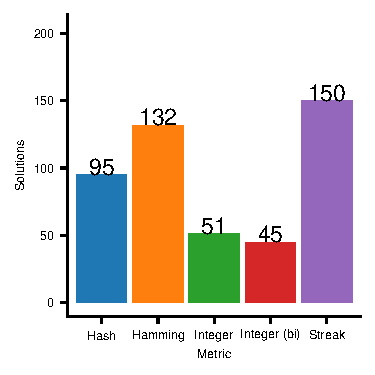
\includegraphics[width=0.75\linewidth]{img/gp_results/panel-dst-sols.pdf}%
\caption{
Numbers of replicates out of 200 that produced a complete solution to the directional-signal task.}
\label{fig:dst-sols}
\end{subfigure}
\begin{subfigure}[b]{\linewidth}
\centering
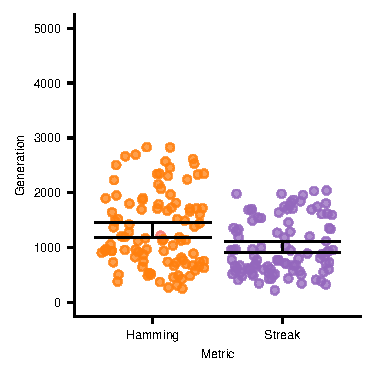
\includegraphics[width=0.75\textwidth]{img/gp_results/panel-dst-times.pdf}%
\caption{
Generations to solution for the first 100 replicates out of 200 to produce a complete solution to the directional-signal task.
Error bars indicate bootstrapped 95\% confidence intervals.
}
\label{fig:dst-times}
\end{subfigure}

\label{fig:gp_results}

\caption{
Evolutionary performance of tag-matching metrics on the directional signals.
All show each metrics' best-performing mutation rate.
}

\label{fig:evo_directional_signal}
\end{figure}
